\section{Inlets e Outlets}


\begin{frame}{Inlets e outlets}
\begin{figure}[ht!]
\centering
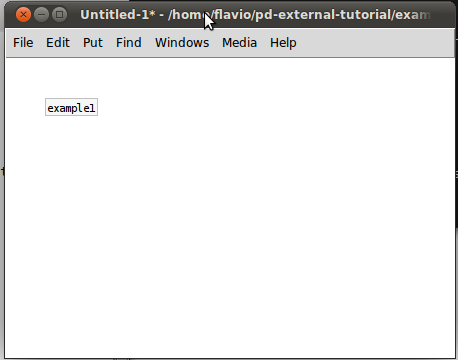
\includegraphics[height=0.6\textheight]{example1}
\caption{Para que serve isso!?}
\end{figure}
\end{frame}


\begin{frame}{Inlets passivos (1/3)}
\begin{figure}[h!]
\centering
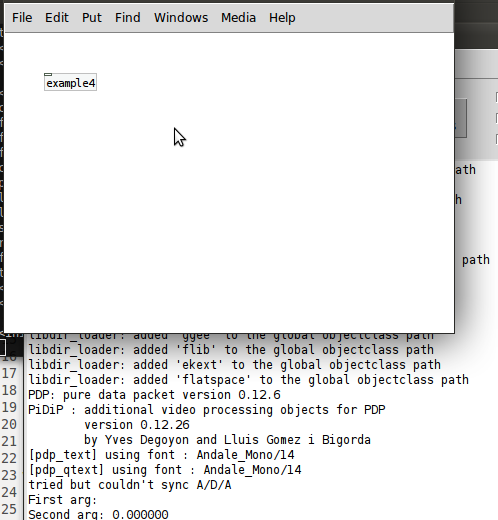
\includegraphics[height=0.8\textheight]{example4}
\label{fig:inlet-passivo}
\end{figure}
\end{frame}


\begin{frame}[fragile]{Inlets passivos (2/3)}
\begin{lstlisting}
static t_class *example4_class;

typedef struct _example4 {
  t_object x_obj;
  t_float my_float;
} t_example4;

// Constructor of the class
void *example4_new(t_symbol *arg1, t_floatarg arg2) {
  t_example4 *x = (t_example4*)pd_new(example4_class);
  post("First arg: %s", arg1->s_name);
  post("Second arg: %f", arg2);
  floatinlet_new(&x->x_obj, &x->my_float);
  return (void *) x;
}
\end{lstlisting}
\end{frame}


\begin{frame}{Inlets passivos (3/3)}
As funções para criar inlets passivos dos tipos mais comuns são:
\begin{itemize}
\item \texttt{floatinlet\_new(t\_object *owner, t\_float *fp)}
\item \texttt{symbolinlet\_new(t\_object *owner, t\_symbol **sp)}
\item \texttt{pointerinlet\_new(t\_object *owner, t\_gpointer *gp)}
\end{itemize}
\end{frame}


\begin{frame}{Inlets ativos (1/2)}
\begin{figure}[h!]
\centering
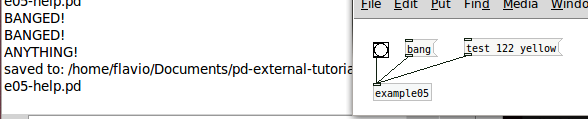
\includegraphics[width=0.7\textwidth]{example5}
\caption{Inlets ativos.}
\label{fig:inlet-ativo}
\end{figure}
\end{frame}


\begin{frame}[fragile]{Inlets ativos (2/2)}
\begin{lstlisting}[language=C]
// inlet-methods receive the object as first argument.
void example5_bang(t_example5 *x) { 
  post("BANGED!");
  post("My_float value: %f",x->my_float);
}

void example5_anything(t_example5 *x, t_symbol *s, int argc, t_atom *argv){
  post("ANYTHING!");
}

void example5_setup(void) {
  example5_class = class_new(gensym("example5"),
    (t_newmethod) example5_new, // Constructor
    0,  sizeof (t_example5), CLASS_DEFAULT,
    0); // LAST argument is ALWAYS zero
  class_addbang(example5_class, example5_bang);
  class_addanything(example5_class, example5_anything);
}
\end{lstlisting}
\end{frame}

\begin{frame}{Tratamento de mensagens (1/4)}
\begin{figure}[h!]
\centering
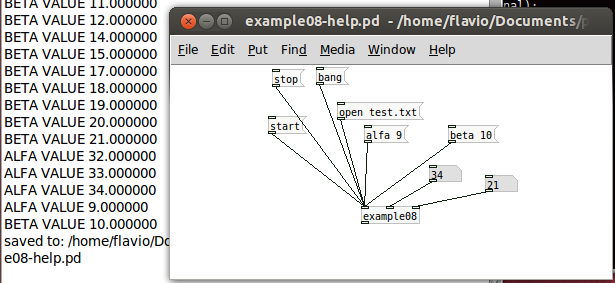
\includegraphics[width=0.7\textwidth]{example8}
\label{fig:inlet-ativo}
\end{figure}
\end{frame}

\begin{frame}[fragile]{Tratamento de mensagens (2/4)}
\lstinputlisting[name=Exemplo 08,linerange=47-61]{../examples/src/example08.c}
\end{frame}


\begin{frame}[fragile]{Tratamento de mensagens (3/4)}
\lstinputlisting[name=Exemplo 08,linerange=17-25,firstnumber=last]{../examples/src/example08.c}
\end{frame}


\begin{frame}[fragile]{Tratamento de mensagens (4/4)}
\lstinputlisting[name=Exemplo 08,linerange=27-45,firstnumber=last]{../examples/src/example08.c}
\end{frame}


\begin{frame}{Outlets (1/4)}
\begin{figure}[h!]
\centering
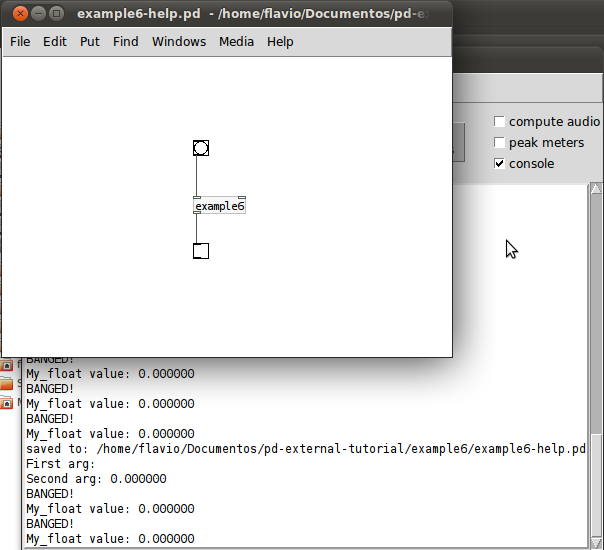
\includegraphics[width=0.7\textwidth]{example6}
\caption{Um external bem útil que recebe um bang e envia um bang.}
\label{fig:outlet-bang}
\end{figure}
\end{frame}


\begin{frame}{Outlets (2/4)}
\lstinputlisting[name=Exemplo 06,linerange=35-45]{../examples/src/example06.c}
\end{frame}


\begin{frame}{Outlets (3/4)}
\lstinputlisting[name=Exemplo 06,linerange=23-33,firstnumber=last]{../examples/src/example06.c}
\end{frame}


\begin{frame}{Outlets (4/4)}
\lstinputlisting[name=Exemplo 06,linerange=6-21,firstnumber=last]{../examples/src/example06.c}
\end{frame}

